\clearpage

\lehead[]{\normalfont\sffamily\hspace*{-2.00cm}\textcolor{white}{\colorbox{lightblue}{\parbox[c][0.70cm][b]{1.60cm}{
\makebox[1.60cm][r]{\thechapter}\\ \makebox[1.60cm][r]{ÜBUNG}}}}\hspace{0.17cm}\textcolor{lightblue}{\chaptertitle}}
\rohead[]{\textcolor{lightblue}{\chaptertitle}\normalfont\sffamily\hspace*{0.17cm}\textcolor{white}{\colorbox{lightblue}{\parbox[c][0.70cm][b]{1.60cm}{\thechapter\\
ÜBUNG}}}\hspace{-2.00cm}}
%\chead[]{}
\rehead[]{\textcolor{lightblue}{AvHG, Inf, My}}
\lohead[]{\textcolor{lightblue}{AvHG, Inf, My}}

\section{Übungsaufgaben: Protokolle}

\subsection{Aufgabe 1: Vier Gewinnt}

Das Spiel \glqq Vier Gewinnt\grqq\ soll als Client-Server-Anwendung programmiert
werden.

Du hast die Aufgabe auf Papier ein geeignetes Protokoll zu entwerfen, mit dem
der Client und der Server untereinander Daten austauschen können. Ein
Programmierer erklärt dir seinen Plan für die Spieloberfläche:

\begin{quotation}
\noindent
Jeder Spieler sieht auf dem Bildschirm ein Spielbrett mit einer Breite von
sieben und einer Höhe von sechs Feldern vor sich. Beide Spieler dürfen
abwechselnd immer einen runden Stein in eine Spalte das Spielbretts fallen
lassen (entweder durch Mausklick oder in dem sie in einem Eingabefeld die
Spaltennummer eingeben). Der Stein fällt auf das unterste freie Feld der
Spalte. Wenn ein Spieler es schafft vier seiner Steine entweder waagerecht,
senkrecht oder diagonal in eine Reihe zu bekommen, hat er gewonnen. Der
Spieler, der anfängt, hat rote Steine. Der andere Spieler hat gelbe Steine.

\noindent
Neben dem Spielbrett befinden sich zwei Buttons. Mit dem ersten Button kann das
Spiel vorzeitig beendet werden, wenn ein Spieler aufgeben möchte. Mit dem
zweiten Button kann ein neues Spiel begonnen werden. Der Computer entscheidet
per Zufallsgenerator darüber, welcher Spieler anfangen kann und die roten
Steine erhält. Außerdem gibt es für die Spieler eine Chat-Möglichkeit. Es gibt
ein Eingabefeld, in das der Spieler einen Text eintragen kann, den er seinem
Mitspieler schicken möchte. Daneben befindet sich ein Button zum Abschicken der
Nachricht. In einer TextArea werden die vom Mitspieler empfangenen
Nachrichten angezeigt.
\end{quotation}

\begin{compactenum}[a)]
\item Skizziere die Oberfläche des Spiels \glqq Vier Gewinnt\grqq .
\item Entwirf ein geeignetes Protokoll.
\end{compactenum}


\subsection{Aufgabe 2: Schiffe Versenken}

Das Spiel \glqq Schiffe versenken\grqq\ soll als Client-Server-Anwendung
programmiert werden.

\begin{compactenum}[a)]
\item Entwirf eine geeignete Programmoberfläche.
\item Entwirf ein Protokoll, mit dem der Client und der Server untereinander
Daten austauschen können.
\end{compactenum}


\subsection{Aufgabe 3: Veranschaulichung des Schichtenmodells}

Das Beispiel arbeitet nur mit drei Schichten. Die Ausgangssituation besteht in
zwei Wissenschaftlern in Arabien und China, die ein Problem diskutieren wollen.
Beide sprechen nur Ihre Landessprache und auch Dolmetscher, die Arabisch und
Chinesisch können, sind nicht aufzutreiben. Beide suchen sich nun Dolmetscher,
die Englisch können. Der Weg der Nachrichten:

\begin{center}
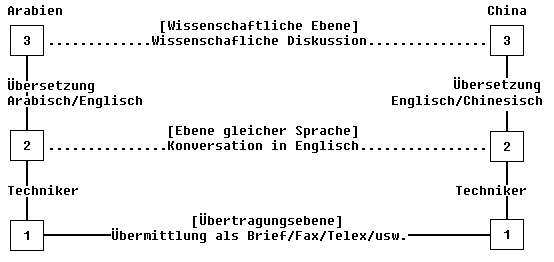
\includegraphics[width=0.75\textwidth]{./inf/SEKII/42_Netzwerke/schichtenmodell_beispiel.png}
% http://www.netzmafia.de/skripten/netze/netz0.html
% Anfrage per e-Mail am 25.3.

Grafik entnommen von \url{http://www.netzmafia.de/skripten/netze/netz0.html}
\end{center}

\subsubsection{Aufgaben}

\begin{compactenum}[a)]
\item Der arabische Wissenschaftler möchte an den chinesischen Wissenschaftler
einen Brief schicken. Beschreibe den Ablauf des Vorgangs.
\item Mit welchen der beteiligten Personen tritt der arabische Wissenschaftler
direkt in Kontakt?
\item Welche Kenntnisse benötigt der arabische Wissenschaftler über den
arabischen Techniker und den chinesischen Techniker?
\end{compactenum}


\subsection{Aufgabe 4: TCP und UDP}

\begin{compactenum}[a)]
\item Der Header des UDP-Protokolls ist recht übersichtlich. Welche zusätzlichen
Informationen muss das TCP-Protokoll in seinen Header packen, damit es die
Inhalte der Datenpakete in der richtigen Reihenfolge zusammenbauen kann und
mitbekommt, ob ein Datenpaket verloren gegangen ist? Da die Datenpakete
verschiedene Wege im Netz nehmen können, kann nicht vorher gesagt werden, in
welcher Reihenfolge die Datenpakete das Ziel erreichen.

\item Warum steht im Header des UDP-Protokolls keine Information über die
Adresse des Rechners, zu dem die Daten gesendet werden sollen?
\end{compactenum}


\section{Übungsaufgaben: IP-Adressen und Ports}

% \subsection{Aufgabe 5: Netzwerk-Klassen}
% 
% Die folgende Tabelle beschreibt die Länge der Netzwerk-ID und der Host-ID für
% die drei verschiedenen Netzwerk-Klassen:
% 
% \begin{center}
% \begin{minipage}{0.95\textwidth}
% \bgroup
% \def\arraystretch{1.2}
% \begin{tabularx}{\textwidth}{|X|X|X|X|}
% \hline
% \textbf{Klasse} & \textbf{A} & \textbf{B} & \textbf{C}
% \\ \hline
% \textbf{Adressbereich} &
% \lstinline|0.0.0.0| bis 
% 
% \lstinline|127.255.255.255| &
% \lstinline|128.0.0.0| bis 
% 
% \lstinline|191.255.255.255| &
% \lstinline|192.0.0.0| bis 
% 
% \lstinline|223.255.255.255|
% \\ \hline
% \textbf{Netzwerk-ID} & 7 Bit & 14 Bit & 21 Bit
% \\ \hline
% \textbf{Host-ID} & 24 Bit & 16 Bit & 8 Bit
% \\ \hline
% \end{tabularx}
% \egroup
% \end{minipage}
% \end{center}
% 
% Berechne die Anzahl der Netze, die es von jedem Netz-Typ gibt, und die Anzahl
% der Rechner, die in einem Netz vom Typ A, B oder C angeschlossen werden können.


\subsection{Aufgabe 5: IP-Adresse des eigenen Rechners}

Ermittle die IP-Nummer deines Rechners. 
% Untersuche mit Hilfe dieser IP-Adresse,
% zu welchem Netz-Typ (A, B oder C) unser Schulnetz gehört.


\subsection{Aufgabe 6: Ports}

\begin{compactenum}[a)]
\item Erkläre was man in der Informatik unter einem Port versteht.

\item Der folgende Text beschreibt, wie Hacker einen PC unter Verwendung der
Ports angreifen können. Beschreibe den Sachverhalt mit deinen eigenen Worten.

\begin{quotation}
\noindent \textbf{Ports -- ein offenes Tor}

\noindent
Jedes Programm, das eine Schnittstelle zum Internet bereit stellt, muss einen
Port (eine Tür) öffnen, damit ihr PC Daten senden und empfangen kann. Ist so
ein Port einmal geöffnet, kann er theoretisch von jedermann (auch
missbräuchlich) benutzt werden. Allerdings kann ein Eindringling, um in diesem
Bild zu bleiben, von außen dieses Tor nicht durchschreiten. Er benötigt einen
\glqq Helfer im Haus\grqq , der für ihn Aufgaben wie Datendiebstahl oder
Sabotage erledigt. Die Anweisungen an den \glqq Helfer\grqq\ oder der Transport
der gestohlenen Daten werden nur durch das geöffnete Tor ermöglicht. Ein
geöffneter Port stellt also immer eine potentielle Gefahr dar.

\noindent
\textbf{Weshalb sind Ports geöffnet und wie kommen die internen \glqq
Helfer\grqq\ in den PC?}

\noindent
Wie oben beschrieben, benötigt das Betriebssystem Ports für die externe
Kommunikation und erledigt bei Anfragen über diese Ports bestimmte Aufgaben.
Einige \glqq Hacker\grqq\ benutzen Insiderkenntnisse und missbrauchen (i.d.R.
bei MS-Windows) das Betriebssystem für kriminelle Zugriffe. Wenn dies möglich
ist, darf man das getrost als schwere Sicherheitslücke bezeichnen.

\noindent
Solche Hacker verbreiten nun Programme, die sich als nette, kleine Spielerei,
als Schutzsoftware oder als kostenfreier Internetzugang usw.\ tarnen.
\myFile{AOL4FREE.EXE} ist so ein Programm. Diese Programme haben oft nur die
eine Aufgabe, sich fest in ihrem System zu installieren und einen Port (als
Hintertür) zu öffnen. Ein Geschenk vom Gegner, das sich später als Falle
herausstellt, kennt man aus der Geschichte als \emph{Trojanisches Pferd}.
Odysseus besiegte mit dieser List die belagerte Stadt Troja. Programme, die
nach dem gleichen Muster arbeiten, bezeichnet man ebenfalls als Trojaner oder
als \glqq Backdoor\grqq , da sie dem Angreifer eine Hintertür öffnen.

\noindent
Entsprechend ihrer Programmierung können solche Trojaner Daten und Programme
zerstören, vertrauliche Daten wie Geschäftsgeheimnisse, Kontonummern,
Passwörter und PINs ausspionieren und damit erheblichen Schaden anrichten.

\noindent
Insgesamt stehen 65535 verschiedene Ports zur Verfügung. 

\noindent
Da es jedem Programmierer letztlich selbst überlassen ist, welchen Port er
nutzt, könnte sich beispielsweise ein Trojaner hinter dem Port 80 verstecken,
solange auf ihrem PC kein Webserver läuft. Port 80 ist ein \emph{well known
Port} und sollte eigentlich nur für die HTTP-Übertragung genutzt werden.
\end{quotation}
\end{compactenum}


\subsection{Aufgabe 7: Programmierübung}

Programmiere ein Java-Frame, das eine vom Benutzer eingegebene Rechner-Adresse
(IP-Nummer oder Domain-Name) vom DNS-Server überprüfen lässt und den vom
DNS-Server ermittelten Namen und die IP-Adresse in zwei Textfeldern ausgibt.
Falls der DNS-Server die Adresse nicht auflösen kann, wird eine Fehlermeldung
ausgegeben.

\begin{center}
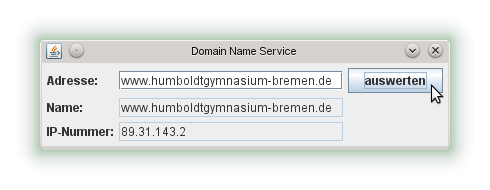
\includegraphics[width=0.8\textwidth]{./inf/SEKII/42_Netzwerke/JavaDNS.png}
\end{center}